Di seguito verranno descritti tutti i test di validazione, di sistema e di integrazione che sono stati previsti. Si prevede in futuro l'aggiornamento dei test di unità. Per le tempistiche di aggiornamento dei test si faccia riferimento al \textit{Piano di Progetto v3.0.0}. La dicitura \textbf{N.A.} contenuta nella colonna \textit{Stato} nelle tabelle sottostanti indica che il test non é ancora stato applicato in quanto verrà applicato solo successivamente, come descritto nel \textit{Piano di Progetto v3.0.0}.


\subsection{Test di sistema}
In questa sezione vengono descritti i test di sistema che permettono di verificare il comportamento dinamico del sistema nella sua interezza rispetto ai requisiti descritti nell'\textit{Analisi dei Requisiti v3.0.0}.
I test di sistema descritti sotto, sono quelli che si riferiscono ai requisisti software individuati e quindi meritevoli di un test.

\subsubsection{Descrizione dei test di sistema}
\begin{center}
	\begin{table}[h]
		\begin{tabular}{|l|p{0.7\textwidth}|l|c|}
			\toprule
			
			\textbf{Test} & \textbf{Descrizione} & \textbf{Stato} & \textbf{Requisito} \\
			
			\midrule
			TS1 & Viene verificato che il sistema registri correttamente un utente & N.A. & R[OBB][F]1\\ \midrule
			TS1.6 & Viene verificato che il sistema registri correttamente un utente attraverso un social network & N.A. & R[OPZ][F]1.6\\ \midrule
			TS2 & Viene verificato che il sistema autentichi correttamente un utente & N.A. & R[OBB][F]2\\  \midrule
			TS3	& Viene verificato che il sistema permetta di effettuare una ricerca di un progetto con le modalità implementate & N.A. & R[OBB][F]3\\ \midrule
			TS4	& Viene verificato che il sistema apra un progetto & N.A. & R[OBB][F]4\\ \midrule
			TS5 & Viene verificato che il sistema generi il PDF del progetto & N.A. & R[OBB][F]5\\ \midrule
			TS6 & Viene verificato che il sistema generi un pacchetto stand-alone per la visualizzazione offline & N.A. & R[OBB][F]6\\ \midrule
			TS7 & Viene verificato che il sistema crei un nuovo progetto & N.A. & R[OBB][F]7\\ \midrule
			TS8 & Viene verificato che il sistema apra un progetto precedentemente creato & N.A. & R[OBB][F]8\\ \midrule
			TS9 & Viene verificato che il sistema permetta la modifica del contenuto di una \gls{slide} & N.A. & R[OBB][F]9\\ \midrule
			TS10 & Viene verificato che il sistema crei un'\gls{infografica} & N.A. & R[DES][F]10\\ \midrule
			TS11 & Viene verificato che il sistema permetta di salvare un progetto & N.A. & R[OBB][F]11\\ \midrule
			TS12 & Viene verificato che il sistema elimini un progetto & N.A. & R[OBB][F]12\\ \midrule
			TS13 & Viene verificato che il sistema permetta di consultare il manuale utente & N.A. & R[OBB][F]13\\
			
						
			\bottomrule
			
		\end{tabular}
		\caption{Tabella di tracciamento test di sistema/requisiti}
		
	\end{table}
	
\end{center}

\newpage

\subsection{Test di integrazione}
In questa sezione vengono descritti i test di integrazione da usare per testare le componenti descritte nella progettazione ad alto livello. Tali test permettono di verificare la corretta implementazione ed il corretto flusso dei dati all'interno del sistema. È stato scelto di utilizzare una strategia di integrazione incrementale, che permette lo sviluppo e la verifica delle componenti in parallelo. Unendo infatti le varie componenti per via incrementale, nella maggior parte dei casi, gli errori riscontrati da un test sono da attribuirsi all'ultima parte aggiunta, inoltre con questa strategia é possibile retrocedere e tornare ad uno stato noto e funzionante del sistema. Si é deciso di utilizzare il metodo bottom-up per integrare prima le componenti con minori dipendenze funzionali e maggiori funzionalità (che corrispondono alle componenti per garantire i requisiti obbligatori) al fine di ottenere il prima possibile una versione funzionante delle parti obbligatorie del sistema. Agendo in questo modo le componenti strettamente legate a parti obbligatorie vengono testate molte volte contribuendo così ad abbassare il numero di errori in esse contenute. Si procede poi risalendo l'albero delle dipendenze fino ad arrivare alla componente di alto livello alla quale saranno dedicati gli ultimi test.

\begin{figure}[h]
\centering
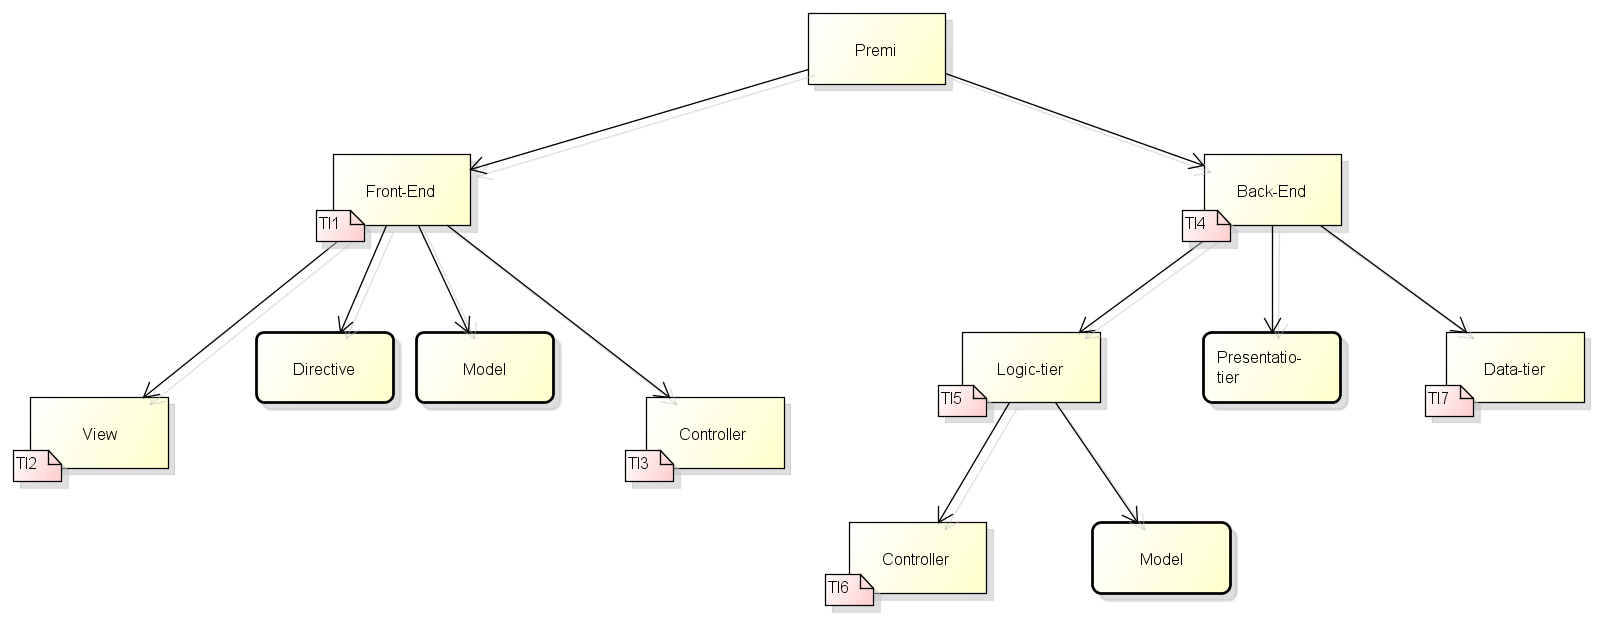
\includegraphics[width=1\linewidth]{img/Integrazione_componenti.png}
\caption[Sequenza d'integrazione delle componenti]{Sequenza d'integrazione delle componenti}
\label{fig:Integrazione_componenti}
\end{figure}

\subsection{Descrizione dei test di integrazione}


\begin{center}
	\begin{table}[h]
		\begin{tabular}{|l|p{0.7\textwidth}|l|c|}
		\toprule
			\textbf{Test} & \textbf{Descrizione} & \textbf{Componente} & \textbf{Stato} \\
			\midrule
			TI1 & Test di controllo finale lato utente & Front-End & N.A\\
			\midrule
			TI2 & Test che verifica la corretta visualizzazione delle interfacce & View & N.A\\
			\midrule
			TI3 & Test che verifica la corretta interazione tra i comandi & Controller & N.A\\
			\midrule
			TI4 & Test che verifica il corretto comportamento tra client e server & Back-End & N.A\\
			\midrule
			TI5 & Test che verifica il corretto funzionamento del server & Logic-tier & N.A\\
			\midrule
			TI6 & Test che verifica la corretta interazione tra i comandi del server & Controller & N.A\\
			\midrule
			TI7 & Test che verifica la correttezza dei dati & Back-End::Data-tier & N.A\\
		\bottomrule
		\end{tabular}
		\caption{Tabella di tracciamento test di integrazione}
	\end{table}
\end{center}
\newpage
\subsection{Tracciamento componenti–test di integrazione}
\begin{table}[h]
	\begin{center}
	\begin{tabular}{|c|c|}
	\toprule
		\textbf{Componente} & \textbf{Test}\\
	\midrule
		Front-End & TI1\\
	\midrule
		Front-End::View & TI2\\
	\midrule
		Front-End::Controller & TI3\\
	\midrule
		Back-End & TI4\\
	\midrule
		Back-End::Logic-tier & TI5\\
	\midrule
		Back-End::Logic-tier::Controller & TI6\\
	\midrule
		Back-End::Data-tier & TI7\\
	\bottomrule
	\end{tabular}
	\end{center}
	\caption{Tabella di tracciamento test di integrazione}
\end{table}


\subsection{Test di validazione}
In questa sezione si descrivono i test di validazione che servono per accertarsi che il prodotto realizzato sia conforme alle aspettative.
Per ogni test vengono descritti i vari passi che un utente deve eseguire per testare i requisiti ad esso associati. Per quanto riguarda il tracciamento test di validazione/requisiti é riportato in \textit{Analisi dei Requisiti v3.0.0}.

\subsubsection{Test TV1}
L'utente vuole verificare che ci si possa iscrivere, anche tramite un social network. \newline
All'utente é richiesto di:
\begin{itemize}
	\item Inserire un nome utente univoco (TV1.1);
	\item Inserire una password di almeno 8 caratteri (TV1.2);
	\item Inserire il proprio nome (TV1.3);
	\item Inserire il proprio cognome (TV1.4);
	\item Inserire il proprio indirizzo email (TV1.5);
	\item Confermare i dati inseriti e controllare di aver ricevuto un messaggio di avvenuta registrazione (TV1.6);
	\item Se i dati inseriti sono sbagliati visualizzare un messaggio di errore (TV1.7).
\end{itemize}

\subsubsection{Test TV2}
L'utente vuole verificare che ci si possa autenticare. \newline
All'utente é richiesto di:
\begin{itemize}
	\item Inserire il proprio nome utente (TV2.1);
	\item Inserire la propria password (TV2.2);
	\item Confermare i dati inseriti cliccando il bottone "Accedi" e visualizzare il messaggio di esito dell'operazione (TV2.3);
	\item Se le credenziali sono errate, premere il bottone per il recupero dei dati (TV2.4);
	\item Inserire la mail usata durante la registrazione (TV2.5);
	\item Se le credenziali sono corrette, controllare di poter accedere alla propria pagina personale (TV2.6).
\end{itemize}

\subsubsection{Test TV3}
L'utente vuole verificare di riuscire a visualizzare i risultati di una ricerca. \newline
All'utente é richiesto di:
\begin{itemize}
	\item Effettuare una ricerca usando come chiave un nome utente (TV3.1);
	\item Effettuare una ricerca usando come chiave un titolo di un progetto (TV3.2);
	\item Verificare che compaia la lista dei risultati della ricerca (TV3.3);
	\item Cambiare nome utente e effettuare una nuova ricerca (TV3.4);
	\item Cambiare titolo del progetto e effettuare una nuova ricerca (TV3.5).
\end{itemize}

\subsubsection{Test TV4}
L'utente vuole verificare di riuscire a visualizzare una presentazione o un'infografica. \newline
All'utente é richiesto di:
\begin{itemize}
	\item Aprire una presentazione (TV4.1);
	\item Scegliere l'opzione per la visualizzazione come ascoltatore (TV4.2);
	\item Scegliere l'opzione per la visualizzazione come presentatore (TV4.3);
	\item Verificare che la presentazione sia visualizzata correttamente e che ci si possa muovere liberamente tra le \gls{slide} (TV4.4);
	\item Verificare che vengano visualizzati gli aiuti a schermo se si ha scelto la visualizzazione come presentatore (TV4.5);
	\item Scegliere di aprire un'infografica e verificare che venga visualizzata (TV4.6).
\end{itemize}


\subsubsection{Test TV5}
L'utente vuole verificare che si possa creare il PDF da una presentazione o da un'infografica. \newline
All'utente é richiesto di:
\begin{itemize}
	\item Scegliere di generare il PDF di una presentazione dall'apposito menù (TV5.1);
	\item Scegliere di generare il PDF di un'infografica dall'apposito menù (TV5.2).
\end{itemize}

\subsubsection{Test TV6}
L'utente vuole verificare che il progetto possa essere esportato in un pacchetto stand-alone per la visualizzazione offline. \newline
All'utente é richiesto di:
\begin{itemize}
	\item Scegliere la posizione in cui salvare il progetto in locale (TV6.1).
\end{itemize}

\subsubsection{Test TV7}
L'utente vuole verificare che si possa creare un nuovo progetto. \newline
All'utente é richiesto di:
\begin{itemize}
	\item Inserire un titolo (TV7.1);
	\item Scegliere un template (TV7.2).
\end{itemize}

\subsubsection{Test TV8}
L'utente vuole verificare che si possa aprire un progetto salvato. \newline
All'utente é richiesto di:
\begin{itemize}
	\item Selezionare il progetto da aprire (TV8.1).
\end{itemize}

\subsubsection{Test TV9}
L'utente vuole verificare che si possa modificare una slide, inserendo, modificando o eliminando un elemento. \newline
All'utente é richiesto di:
\begin{itemize}
	\item Cambiare il template (TV9.1);
	\item Inserire una slide nella posizione che preferisce (TV9.2);
	\item Rimuovere una slide (TV9.3);
	\item Modificare una slide (TV9.4);
	\item Inserire un'immagine (TV9.5);
	\item Inserire del testo o modificare del testo già esistente (TV9.6);
	\item Inserire dei dati real time, possibilmente anche da file (TV9.7);
	\item Inserire una tabella o modificarne una già esistente (TV9.8);
	\item Inserire un grafico o modificarne uno già esistente (TV9.9);
	\item Scegliere un effetto di transizione (TV9.10);
	\item Modificare l'aspetto di un elemento (TV9.11);
	\item Rimuovere un elemento (TV9.12);
	\item Cambiare posizione ad un elemento (9.13);
	\item Caricare un file da inserire (TV9.14).
\end{itemize}

\subsubsection{Test TV10}
L'utente vuole verificare che si possa creare un'infografica. \newline
All'utente é richiesto di:
\begin{itemize}
	\item Scegliere aspetto e contenuti dell'infografica (TV10.1).
\end{itemize}

\subsubsection{Test TV11}
L'utente vuole verificare che si possa salvare un progetto. \newline
All'utente é richiesto di:
\begin{itemize}
	\item Premere il bottone di salvataggio (TV11.1);
	\item Scegliere un nome da dare al progetto (TV11.2).
\end{itemize}

\subsubsection{Test TV12}
L'utente vuole verificare che si possa eliminare un progetto. \newline
All'utente é richiesto di:
\begin{itemize}
	\item Selezionare il progetto da eliminare (TV12.1);
	\item Confermare l'eliminazione (TV12.2).
\end{itemize}